 \subsubsection{UC5 - Visualizzazione beni}
 \begin{figure}[h]
 	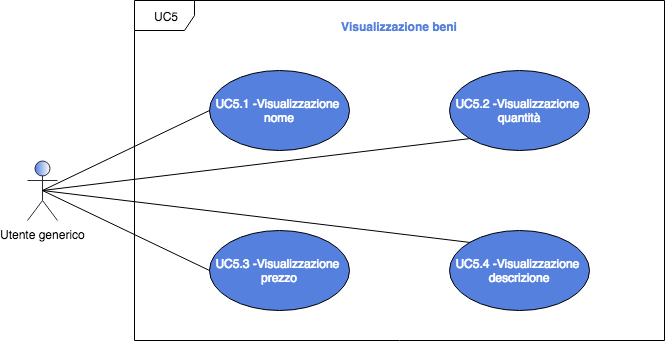
\includegraphics[width=10cm]{res/images/UC5VisualizzazioneBeni.png}
 	\centering
 	\caption{UC5 - Visualizzazione beni}
 \end{figure}
 \begin{itemize}
 	\item \textbf{Attori Primari}: utente generico;
 	\item \textbf{Descrizione}: l'utente visualizza una lista dettagliata di informazioni relative ad un bene o servizio;
 	\item \textbf{Scenario}: l'utente si trova all'interno della pagina di un bene o servizio e può trarre le seguenti informazioni:
 		\begin{enumerate}[label=\alph*.]
 		\item visualizzazione nome [UC5.1];
 		\item visualizzazione quantità [UC5.2];
 		\item visualizzazione prezzo [UC5.3];
 		\item visualizzazione descrizione [UC5.4];
 	\end{enumerate}
 	\item \textbf{Precondizione}: l'utente, navigando nel sito, risulta all'interno della pagina di un bene o servizio;
 	\item \textbf{Postcondizione}: l'utente può procedere all'acquisto del bene o del servizio, se loggato.
 \end{itemize}
 \subsubsection{UC5.1 - Visualizzazione nome}
\begin{itemize}
	\item \textbf{Attori Primari}: utente generico;
	\item \textbf{Descrizione}: l'utente visualizza il nome del bene o del servizio;
	\item \textbf{Scenario}: l'utente si trova all'interno della pagina di un bene o servizio;
	\item \textbf{Precondizione}: l'utente ha espresso la volontà di visualizzare la pagina di un bene o un servizio;
	\item \textbf{Postcondizione}: l'utente conosce il nome del prodotto.
\end{itemize}
 \subsubsection{UC5.2 - Visualizzazione quantità}
\begin{itemize}
	\item \textbf{Attori Primari}: utente generico;
	\item \textbf{Descrizione}: l'utente visualizza la quantità del bene o del servizio selezionato;
	\item \textbf{Scenario}: l'utente si trova all'interno della pagina di un bene o servizio;
	\item \textbf{Precondizione}: l'utente ha espresso la volontà di visualizzare la pagina di un bene o un servizio;
	\item \textbf{Postcondizione}: l'utente è consapevole del fatto che la quantità visualizzata saà quella che, se vorrà, inserirà nel carrello.
\end{itemize}
 \subsubsection{UC5.3 - Visualizzazione prezzo}
\begin{itemize}
	\item \textbf{Attori Primari}: utente generico;
	\item \textbf{Descrizione}: l'utente visualizza il prezzo del bene o del servizio;
	\item \textbf{Scenario}: l'utente si trova all'interno della pagina di un bene o servizio;
	\item \textbf{Precondizione}: l'utente ha espresso la volontà di visualizzare la pagina di un bene o un servizio;
	\item \textbf{Postcondizione}: l'utente conosce il prezzo del prodotto.
\end{itemize}
 \subsubsection{UC5.4 - Visualizzazione descrizione}
\begin{itemize}
	\item \textbf{Attori Primari}: utente generico;
	\item \textbf{Descrizione}: l'utente visualizza la descrizione del bene o del servizio;
	\item \textbf{Scenario}: l'utente si trova all'interno della pagina di un bene o servizio;
	\item \textbf{Precondizione}: l'utente ha espresso la volontà di visualizzare la pagina di un bene o un servizio;
	\item \textbf{Postcondizione}: l'utente conosce la descrizione del prodotto.
\end{itemize}